\section*{Collector: Efficient selection of devices to request file download}

In a peer-to-peer configuration of devices that share a store, through the
consistency algorithm of the base system~\cite{wang:patent2012}, updates to
objects are propagated among devices. In this context, receipt of an update for
object with id $o$ (from the perspective of ``this" local device) signifies that
the device now has knowledge that some modification, creation, renaming, or
deletion of $o$ occurred on some other device in the network. Given this update
knowledge, and assuming the local device knows all those that are online, how
can the local device choose from which of its peers to download that update? The
Collector algorithm defines a set of steps to convert known missing updates into
locally downloaded files or folders, without naively querying every device for
the update until one succeeds. This latter approach would waste bandwidth and
computation by potentially querying devices that do not have the update. For
example, suppose a network has three devices sharing files, $d_1, d_2, d_3$.
Device $d_3$ modifies object $o$, which propagates updates to $d_1$ and $d_2$.
Upon receipt of that update for $o$, $d_1$ should only request to download the
change from $d_3$, not wasting bandwidth and CPU resources by requesting from
$d_2$.

The claimed algorithm records and shares, among peers, which updates each device
has observed in the distributed system. The algorithm will determine, and query
from, the set of devices that are known to have the update. Given the set of
devices known to have the update, the algorithm selects devices to query in
order of preference based on a device's network bandwidth, workload, etc.

\subsection*{Data Structures}

\subsubsection*{Sharing existence of local updates}

There exists locally, for every device $d$ known to this local device, two sets
of object ids: $S_{xd}$ is the set of objects updated since the last version
exchange between the local and $d$. The other, $S_{hd}$, is the set of all other
objects updated on the local device. The two sets are disjoint and their union
represents all objects with updates downloaded on this device. After performing
an update locally on an object, the local device adds the object to the $S_{xd}$
set, for every known remote device.

When responding to a pull version request~\cite{wang:patent2012} from a remote
device $d$, the local device additionally sends the set above, $S_{xd}$, of
locally recorded updates. The remote device $d$ will respond with success or
failure. On receipt of a success message, the local device unions $S_{xd}$ with
$S_{hd}$, which records all objects ever updated at this device, then empties
the $S_{xd}$ set. Thus $S_{xd}$ acts as a ``diff" of objects updated between
version exchanges of the local device and $d$.

\subsubsection*{Collector sets}

\begin{figure}[t]
\centering
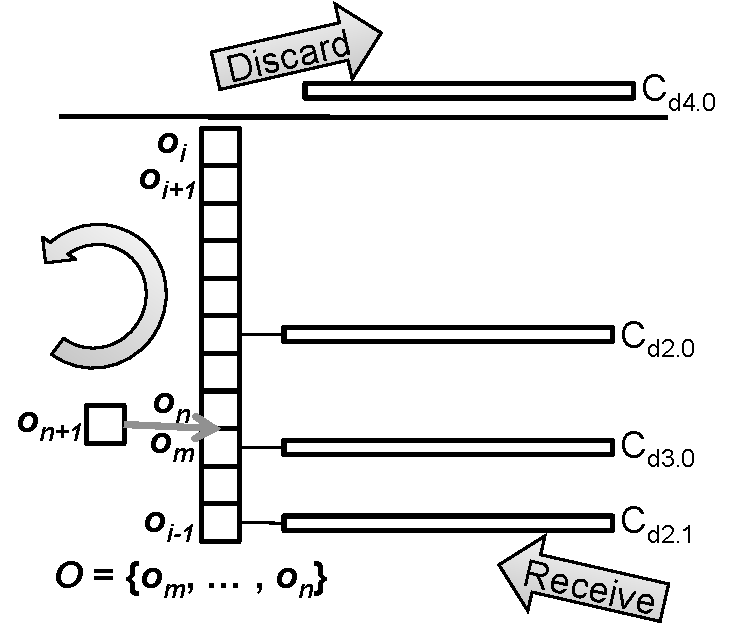
\includegraphics{figs/collector.pdf}
\caption{Collector Diagram}
\label{fig:collectorferris}
\end{figure}

In Figure~\ref{fig:collectorferris}, a set of objects, $O=\{o_m,\ldots,o_n\}$,
is pictured as a vertical queue with $o_i$ currently at the head, and $o_{i-1}$
at the tail, where $1 \leq m \leq i \leq n$. These objects are known to have
updates on remote devices, and are {\em collected} by cycling through the queue.
Collecting an object involves requesting and downloading the update from a
remote device (not covered in this patent). The goal of this algorithm is to
collect updates for all objects in $O$ by contacting only those devices which
actually have any given update available. The queue wraps the $O$ set, giving
the objects a particular order, where their {\em sequence numbers} are
monotonically increasing---object $o_i$ has sequence number $i$ and therefore
precedes $o_{i+1}$. Object $o_n$ is adjacent to $o_m$, where $m$ is the minimum
sequence number among the objects in $O$; $m$ could take value 1, but objects
are also removed from this queue. The current object to be collected is $o_i$ at
the head of the queue.

Also pictured in Figure~\ref{fig:collectorferris} are the sets $C_{di.t}$ as long
rectangles. Whereas sets $S_x$ and $S_h$ (described above) record updates the
local device has observed, the Collector algorithm relies upon the set $C_d$,
which represents the objects for which device $d$ has updates (i.e. the $S_x$
from $d$). Generally, there exists locally, for every device $d$ known to the
local device, one or more sets $C_{d.t}$, which were recorded locally as a
result of exchanging versions for updates with device $d$. Because multiple
version exchanges can occur with the local device and $d$, more than one of
these sets may have been sent.

The set of sets is hereafter called the Collector Sets, or $CS=\{C_{d1.0},
C_{d1.1}, \ldots, C_{dp.0}, C_{dp.1}, \ldots C_{dp.tp}\}$. As seen in the
figure, each set $C_{d.t}$ is assigned to some index in the object queue, $O$. A
newly-received $C$ is assigned to the tail at the bottom of the queue (e.g.
$C_{d2.1}$) in the Figure). There is no relation between $C$, and the object
which shares the same index; this association is intended to safely discard the
sets when their use is expired. It is possible that more than one $C$ set could
be assigned to the same index, representing sets of objects from distinct
devices. The reader may note that when receiving several sets from device $d$,
the incoming set could be unioned with the locally-present $C_d$. This approach
is not taken so that $CS$ can be more easily pruned: if $C_{d.t}$ sets remain
separated, then an older set could be discarded while keeping the
recently-received collector sets. The details of receiving a set $C_d$ from
remote device $d$ is discussed below.

\subsection*{Method to collect updates efficiently}

Given the aforementioned data structures, the Collector algorithm is described
to collect the updates for each object in $O$, by contacting only those devices
known to have a given update. The basic idea is that the set of devices to
contact for object $o \in O$ is determined by querying for the existence of $o$
in each $C$ set. To determine the set of devices, $D$, known to have updates for
$o$:
\begin{algorithmic}
\Function{GetDevicesWithUpdates}{$o$: object id, $CS$: Collector Sets}
\State $D \gets \emptyset$
\For{$C_d \in CS$}
  \If{$o \in C_d$}
    \State $D \gets D \cup \{d\}$
  \EndIf
\EndFor
\State \Return $D$
\EndFunction
\end{algorithmic}

To efficiently collect all objects in $O$, the local device ``rotates" through
the objects of the queue and downloads updates from the set of devices, $D$,
returned by the algorithm above for each object. The local device discards the
object sets $\{C\}$ that are linked to the object popped from the head of $O$,
as all elements in $O$ that could appear in $C$ have already been queried. If
collection of some object $o$ succeeds, the object $o$ is removed from the
queue.
\begin{algorithmic}
\Function{CollectAllUpdates}{$CS$: Collector Sets, $O$: object queue}
\State $CS_{bkup} \gets CS$
\While{$O$ is not empty and $CS$ is not empty}
 \State $o\gets$ pop the head of queue $O$
 \State $D\gets$ GetDevicesWithUpdates($o$)
 \State download updates for $o$ from any device in $D$ until successful
 \State $CS_o \gets$ subset of $CS$ linked to $o$
 \For{$C \in CS_o$}
     \State remove $C$ from $CS$
 \EndFor
 \If{failed in downloading all updates for $o$}
    \State push $o$ to the tail of queue $O$
    \For{$d \in D$}
      \For{$C_d \in CS_{bkup}$ where $C_d$ was received from $d$}
          \State $CS \gets CS \cup \{C_d\}$
      \EndFor
    \EndFor
 \EndIf
\EndWhile
\EndFunction
\end{algorithmic}
Observe that on failure of downloading all updates for $o$ from all devices in
$D$, the sets received from devices in $D$ are restored from $CS_{bkup}$. See
below for details on how a set is inserted into the Collector Sets.

\subsection*{Populating the Object Set and Collector Sets}

\subsubsection*{Insertion to the object queue}
Concurrent with the collection loop execution in CollectAllUpdates, the
consistency algorithm could receive knowledge of new updates for some object
$o$. If the object is not already in $O$, it must be inserted, but not at the
tail as in a conventional queue. To maintain the monotonic property of sequence
numbers in $O$, the new object $o$ is assigned a sequence number of $n+1$, and
is consequently inserted into the queue following $o_n$ (as seen in
Figure~\ref{fig:collectorferris}).
%TODO explain why the monotonic property is required
%TODO explain why this is safe as Mark and Weihan discussed Jan 23.

\subsubsection*{Insertion to the collector sets}

Following a push or pull version exchange from device $d$, a Collector Set $C_d$
is additionally received or created on the local device. The following
pseudocode adds a non-empty $C_d$ to the $CS$ set. An empty $C_d$ can be
ignored.
\begin{algorithmic}
\Function{AddToCollectorSets}{$C_d$: collector set from $d$, $CS$: collector
sets, $O$: object queue}
  \State $CS \gets CS \cup \{C_d\}$
  \State $o_t \gets$ tail of $O$
  \If{$\exists C_c \in CS$ where $C_c$ shares sequence number $t$ and $c == d$}
    \State $C_c \gets C_c \cup C_d$
  \Else
    \State link $C_d$ to $o_t$
  \EndIf
\EndFunction
\end{algorithmic}
Note that multiple $C_d$ sets could be linked to the same object in the $O$
queue, if the queue did not rotate between calls to AddToCollectorSets.

Upon receipt of a push version update from device $d$, after recording versions
locally, the local device creates an object set $C_d$ of all objects with new
updates in the given versions. If all updates for some object $o$ were already
known locally, object $o$ is not added to $C_d$. If $C_d$ is non-empty,
AddToCollectorSets is executed on the set.

Upon receipt of a pull version response from device $d$, the local device first
records the versions locally, including stable and unstable versions (see the
patent~\cite{wang:patent2012} for description of stable and unstable). As
indicated earlier, device $d$ sent its set $S_x$ of updated objects. These
objects have updates on $d$ that are new since the last pull version exchange
made with $d$ from this device. If the received $S_x$ is non-empty, the local
device records it as $C_d$, and executes AddToCollectorSets on it. The local
device subsequently responds to device $d$, indicating successful receipt of the
set $C_d$.

%TODO clean up details from word doc:
%\begin{itemize}
%\item Ordered versions have to be fetched together with the BF in an atomic operation,
%to prevent the case that an ordered KML version is received from P after the
%collector disposes BF.
%\item the versions P must include unordered versions. Otherwise the
%receiver may have disposed P’s BF when receiving an unordered version from P.
%\item Discuss Sender Filter Update Sequence numbers?
%\end{itemize}

\subsection*{Implementation Details}

\subsubsection*{Bloom filter optimization}
In one embodiment of the invention, the sets $S_h$ and $S_x$ (and consequently
the $C$ sets of $CS$) are implemented as Bloom filters~\cite{bloom:cacm70} of
length 1024 bits and four hash functions. The hash functions are disjoint bit
selections from the 128-bit UUID object id. The $CS$ Collector Sets is thus a
set of Bloom filters. This implementation of the object id sets permits
\begin{itemize}
 \item constant-space transmission of object id sets
 \item constant-time membership query of the collecting object in $O$, in each
Bloom filter of $CS$.
\end{itemize}

The negative consequence of replacing accurate sets with Bloom filters is that
the inherent membership query false positives would suggest that a device could
request to download an update from a device that does not have the update
locally. This results in some bandwidth waste, but the algorithm remains
correct, as the requested device can respond with a NACK.
% TODO describe permanent errors briefly here

%\subsubsection*{Invoking the collection loop}
%\subsubsection*{Database persistence of $CS$ and $O$}
%\subsubsection*{Asynchronous/concurrent downloads}
%\subsubsection*{Expulsion/Readmission}
